\hypertarget{a00338}{}\section{Sidechain Inputs}
\label{a00338}\index{Sidechain Inputs@{Sidechain Inputs}}
Routing custom audio streams to a plug-\/in. 

\hypertarget{a00338_additionalFeatures_Sidechain_overview}{}\subsection{Overview of Sidechain Inputs}\label{a00338_additionalFeatures_Sidechain_overview}
If applicable, plug-\/ins may choose to enable sidechain inputs. If a sidechain is enabled, a menu is added to the plug-\/in\textquotesingle{}s header that allows the user to choose an interface or bus as the sidechain, or \char`\"{}key input\char`\"{}. Once enabled, the plug-\/in will be able to access sidechain input just like any other input signal. Currently, D\+A\+E is limited to mono sidechain inputs.\hypertarget{a00338_additionalFeatures_Sidechain_adding}{}\subsection{Adding a Sidechain Input to an Effect}\label{a00338_additionalFeatures_Sidechain_adding}
Setting up a sidechain input is fairly straight forward. You will want to add a physical address within your context structure, and then \char`\"{}describe\char`\"{} the sidechain in Describe.

Context Structure\+:


\begin{DoxyCode}
\textcolor{comment}{//=============================}
\textcolor{comment}{// Component context definitions}
\textcolor{comment}{//=============================}

\textcolor{comment}{// Context structure}
\textcolor{keyword}{struct }SMyPlugIn\_Alg\_Context
\{
   [...]
   int32\_t  * mSideChainP;
   [...]
\};

\textcolor{comment}{// Physical addresses within the context}
\textcolor{keyword}{enum} EDemoDist\_Alg\_PortID
\{
    [...]
    ,MyPlugIn\_AlgFieldID\_SideChain  = \hyperlink{a00149_acf807247ecd6e5899dc9dc31644e9a1d}{AAX\_FIELD\_INDEX} (SDemoDist\_Alg\_Context, mSideChainP)
    [...]
\};
\end{DoxyCode}


Describe\+: 
\begin{DoxyCode}
\textcolor{comment}{// ***************************************************************************}
\textcolor{comment}{// ROUTINE: DescribeAlgorithmComponent}
\textcolor{comment}{// Algorithm component description}
\textcolor{comment}{// ***************************************************************************}
\textcolor{keyword}{static} \textcolor{keywordtype}{void} DescribeAlgorithmComponent( \hyperlink{a00088}{AAX\_IComponentDescriptor} * outDesc )
\{
    \hyperlink{a00149_a4d8f69a697df7f70c3a8e9b8ee130d2f}{AAX\_Result}                    err = \hyperlink{a00207_a5f8c7439f3a706c4f8315a9609811937aeddbd1bb67e3a66e6af54a4b4a7a57b3}{AAX\_SUCCESS};

    [...]
    err = outDesc.\hyperlink{a00088_a1e0c9508d1eb0c9a60a87a0fb69f1dbe}{AddSideChainIn}(eDemoDist\_AlgFieldID\_SideChain);
    [...]
    properties->\hyperlink{a00112_a0997671afce9a2367662c764c1d055dd}{AddProperty} ( \hyperlink{a00283_a6571f4e41a5dd06e4067249228e2249ea3399fcd8ff459de1e3de0c98d40a5094}{AAX\_eProperty\_SupportsSideChainInput}
      , \textcolor{keyword}{true} );
    [...]
\}
\end{DoxyCode}


\begin{DoxyRefDesc}{Todo}
\item[\hyperlink{a00382__todo000001}{Todo}]Is properties-\/$>$Add\+Property ( A\+A\+X\+\_\+e\+Property\+\_\+\+Supports\+Side\+Chain\+Input, true ) even necessary?!?! I believe I saw a p.\+i. that does not declare this...\end{DoxyRefDesc}


In order to tell whether there is sidechain information available to your plug-\/in, check for a null pointer within your algorithm\textquotesingle{}s process function. The sidechain channel will show up as an additional stem from the original stem format you declare. That is to stay, for a stereo plug-\/in, the sidechain channel will be the third channel passed in.


\begin{DoxyCode}
\textcolor{comment}{//==============================================================================}
\textcolor{comment}{// Processing function definition}
\textcolor{comment}{//==============================================================================}

\textcolor{keywordtype}{void}
\hyperlink{a00149_aaa22112139aa627574b1ef562f579d43}{AAX\_CALLBACK}
MyPlugIn\_AlgorithmProcessFunction (
    SMyPlugIn\_Alg\_Context * \textcolor{keyword}{const}   inInstancesBegin [],
    \textcolor{keyword}{const} \textcolor{keywordtype}{void} *                    inInstancesEnd)
\{
    [...]
    int32\_t sideChainChannel = *instance->mSideChainP;   
    \textcolor{keywordtype}{float} * AAX\_RESTRICT sideChainInput = 0;
    \textcolor{keywordflow}{if} ( sideChainChannel )
      sideChainInput = instance->mInputPP [sideChain]Channel;
    [...]
\}
\end{DoxyCode}
 Collaboration diagram for Sidechain Inputs\+:
\nopagebreak
\begin{figure}[H]
\begin{center}
\leavevmode
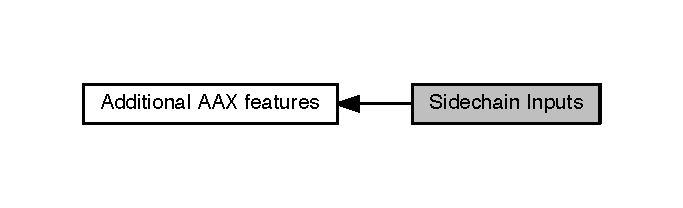
\includegraphics[width=328pt]{a00338}
\end{center}
\end{figure}
